\subsection{Boot Sequence}
\begin{frame}
  \frametitle{Bootloaders}
  \begin{itemize}
  \item The bootloader is a piece of code responsible for
    \begin{itemize}
    \item Basic hardware initialization
    \item Loading of an application binary, usually an operating
      system kernel, from flash storage, from the network, or from
      another type of non-volatile storage.
    \item Possibly decompression of the application binary
    \item Execution of the application
    \end{itemize}
  \item Besides these basic functions, most bootloaders provide a
    shell with various commands implementing different operations.
    \begin{itemize}
    \item Loading of data from storage or network, memory inspection,
      hardware diagnostics and testing, etc.
    \end{itemize}
  \end{itemize}
\end{frame}

\begin{frame}
  \frametitle{Booting on MTK SoC}
  \begin{columns}
    \column{0.3\textwidth}
    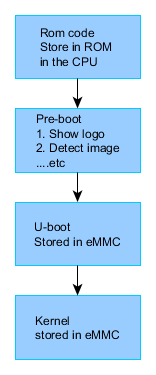
\includegraphics[width=\textwidth]{slides/sysdev-bootloaders-sequence/mtk-boot.png}
    \column{0.7\textwidth}
    \footnotesize
    \begin{itemize}
    \item {\bf ROM Code}: tries to find a valid bootstrap image from
      various storage sources, and load it into RAM. The RAM
      configuration is described in a CPU-specific header, prepended
      to the bootloader image.
	\item {\bf Pre-Boot}: Pre-boot to initialize for Display/Image checking ...etc, and then switch to uboot.
    \item {\bf U-Boot}: runs from RAM. Initializes some other hardware
      devices (network, USB, etc.).  Loads the kernel image from
      storage or network to RAM and starts it. Shell with commands
      provided.
    \item {\bf Linux Kernel}: runs from RAM. Takes over the system
      completely (bootloaders no longer exists).
    \end{itemize}
  \end{columns}
\end{frame}

\begin{frame}
  \frametitle{Generic bootloaders for embedded CPUs}
  \begin{itemize}
  \item We will focus on the generic part, the main bootloader, offering
    the most important features.
  \item There are several open-source generic bootloaders.\\
    Here are the most popular ones:
    \begin{itemize}
    \item {\bf U-Boot}, the universal bootloader by Denx\\
      The most used on ARM, also used on PPC, MIPS, x86, m68k, NIOS,
      etc. The de-facto standard nowadays. We will study it in detail.\\
      \url{http://www.denx.de/wiki/U-Boot}
    \item {\bf Barebox}, a new architecture-neutral bootloader, written
      as a successor of U-Boot. Better design, better code, active
      development, but doesn't yet have as much hardware support as U-Boot.\\
      \url{http://www.barebox.org}
    \end{itemize}
  \item There are also a lot of other open-source or proprietary
    bootloaders, often architecture-specific
    \begin{itemize}
    \item RedBoot, Yaboot, PMON, etc.
    \end{itemize}
  \end{itemize}
\end{frame}
